\documentclass[tikz,border=0bp]{standalone}

\usepackage{fontspec}

\setmainfont[
  Path=C:/Windows/Fonts/,
  UprightFont=times.ttf,
  BoldFont=timesbd.ttf,
  ItalicFont=timesi.ttf,
  BoldItalicFont=timesbi.ttf
]{Times New Roman}

\begin{document}
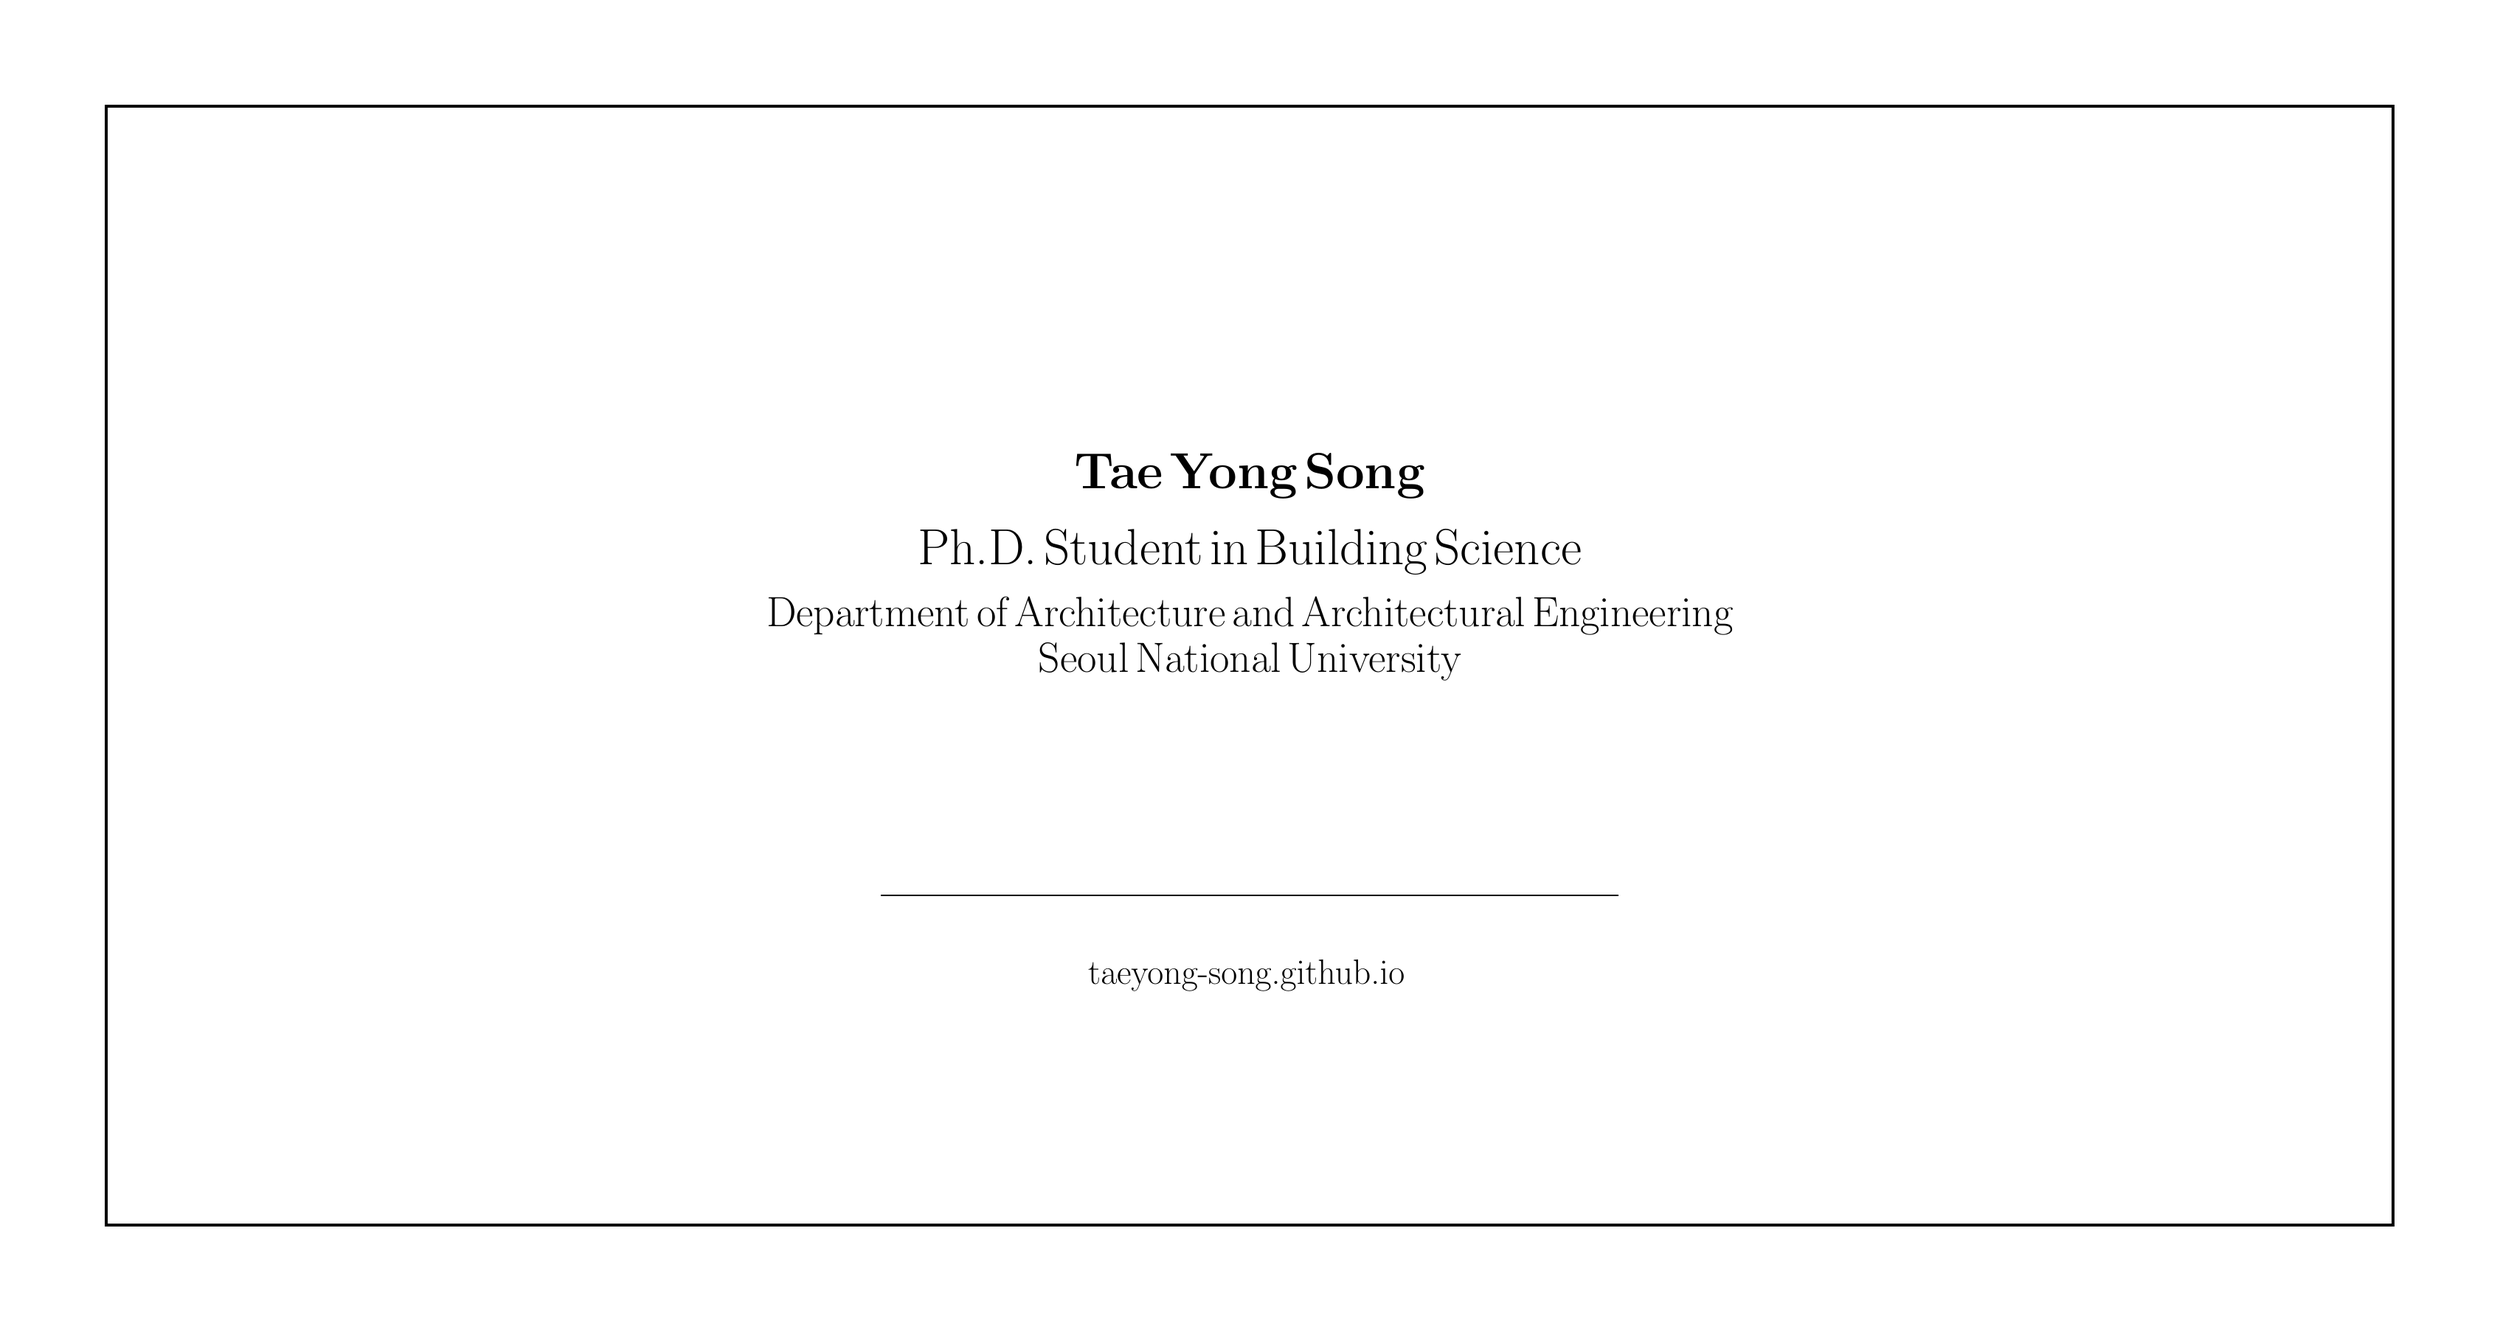
\begin{tikzpicture}[x=1bp,y=1bp]
  \path[use as bounding box] (0,0) rectangle (1200,630);
  \fill[white] (0,0) rectangle (1200,630);
  \draw[black,line width=1.5bp] (42,42) rectangle (1158,588);

  \node[align=center,text width=1040bp] at (600,363) {
    {\fontsize{58}{66}\selectfont\bfseries Tae Yong Song}\\[14bp]
    {\fontsize{27}{33}\selectfont Ph.D. Student in Building Science}\\[10bp]
    {\fontsize{22}{28}\selectfont Department of Architecture and Architectural Engineering}\\[3bp]
    {\fontsize{22}{28}\selectfont Seoul National University}
  };

  \draw[black,line width=0.8bp] (420,203) -- (780,203);

  \node[align=center] at (600,164) {
    {\fontsize{18}{22}\selectfont taeyong-song.github.io}
  };
\end{tikzpicture}
\end{document}
